%\RequirePackage{atbegshi}
\documentclass{beamer}

\usetheme{Rochester}
\usepackage{amssymb}
%\usepackage[cmex10]{amsmath}
\usepackage{stmaryrd,epsfig,psfrag}
\usepackage[english]{babel}
\usepackage{tikz,pgf,pgfplots}
\pgfplotsset{compat=newest}
\usepgflibrary{shapes}
\usetikzlibrary{%
  arrows,%
  mindmap,%mindmap
  calendar,%calendar
  decorations,%decorations
  snakes,%snakes
  shapes.misc,% wg. rounded rectangle
  shapes.arrows,%
	shapes.callouts, %
  shapes,%
  chains,%
  matrix,%
  positioning,% wg. " of "
  scopes,%
  decorations.pathmorphing,% /pgf/decoration/random steps | erste Graphik
	decorations.text, %
  shadows,%
  backgrounds,%
  fit,%
  petri%
}

% Radius of regular polygons
\newdimen\R
\R=0.8cm

\definecolor{tutorial}{RGB}{50,93,61}


\title{Inference on Markov Chains}
\author{Austin Taghavi, Jyothsna Kurra, and Saurav Sahu}
\institute{Electrical and Computer Engineering \\ Texas A\&M University}

%\setbeamertemplate{footline}[page number]
\setbeamertemplate{navigation symbols}{\textcolor{black}{\insertframenumber / \inserttotalframenumber}}

\begin{document}

\begin{frame}
  \titlepage
\end{frame}


\begin{frame}
\frametitle{Outline}
\begin{itemize}
\item \textbf{Introduction}
\item\vspace{0.5cm} Hidden Markov Models
\item\vspace{0.5cm} Forward Backward Algorithm
\item \vspace{0.5cm} Baum-Welch Algorithm
\item \vspace{0.5cm} Viterbi Algorithm
\item \vspace{0.5cm} Conclusions
\end{itemize}
\end{frame}

\begin{frame}
\frametitle{Markov Property}
\begin{columns}
\column{.43\textwidth}
\begin{itemize}
\item The memoryless property of a stochastic process
\item The conditional probability distribution of future states depends only on the present state
\item Future states, conditioned on the current state, are independent of previous states
\end{itemize}
\column{.55\textwidth}
  \begin{center}
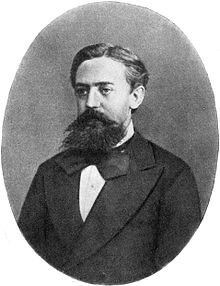
\includegraphics[width=5cm]{Figures/AAMarkov}
  \end{center}
\end{columns}
\end{frame}

\begin{frame}
\frametitle{Outline}
\begin{itemize}
\item Introduction
\item\vspace{0.5cm} \textbf{Hidden Markov Models}
\item\vspace{0.5cm} Forward Backward Algorithm
\item \vspace{0.5cm} Baum-Welch Algorithm
\item \vspace{0.5cm} Viterbi Algorithm
\item \vspace{0.5cm} Conclusions
\end{itemize}
\end{frame}

\begin{frame}
\frametitle{Outline}
\begin{itemize}
\item Introduction
\item\vspace{0.5cm} Hidden Markov Models
\item\vspace{0.5cm} \textbf{Forward Backward Algorithm}
\item \vspace{0.5cm} Baum-Welch Algorithm
\item \vspace{0.5cm} Viterbi Algorithm
\item \vspace{0.5cm} Conclusions
\end{itemize}
\end{frame}

\begin{frame}
\frametitle{Outline}
\begin{itemize}
\item Introduction
\item\vspace{0.5cm} Hidden Markov Models
\item\vspace{0.5cm} Forward Backward Algorithm
\item \vspace{0.5cm} \textbf{Baum-Welch Algorithm}
\item \vspace{0.5cm} Viterbi Algorithm
\item \vspace{0.5cm} Conclusions
\end{itemize}
\end{frame}

\begin{frame}
\frametitle{Outline}
\begin{itemize}
\item Introduction
\item\vspace{0.5cm} Hidden Markov Models
\item\vspace{0.5cm} Forward Backward Algorithm
\item \vspace{0.5cm} Baum-Welch Algorithm
\item \vspace{0.5cm} \textbf{Viterbi Algorithm}
\item \vspace{0.5cm} Conclusions
\end{itemize}
\end{frame}

\begin{frame}
\frametitle{Outline}
\begin{itemize}
\item Introduction
\item\vspace{0.5cm} Hidden Markov Models
\item\vspace{0.5cm} Forward Backward Algorithm
\item \vspace{0.5cm} Baum-Welch Algorithm
\item \vspace{0.5cm} Viterbi Algorithm
\item \vspace{0.5cm} \textbf{Conclusions}
\end{itemize}
\end{frame

\begin{frame}
\frametitle{Conclusions}
\begin{itemize}
\item New framework for a novel problem formulation in the random access space
\item Necessary and sufficient conditions, and methods for deriving transition probabilities
\item Large design space; so far the structure of the problem has not revealed optimal strategies
\item Up to 69 percent efficiency with skewed and stateless distributions
\item Open topics include performance tradeoff with estimating number of users
\end{itemize}
\end{frame}

\begin{frame}
\frametitle{Conclusions}
\begin{itemize}
\item Novel problem formulation, with modified decoding process and bipartite graph
\item Want to balance the number of users at each access point, without having too many overlapping users
\item Should the transmission strategy for overlapping nodes differ? How?
\begin{center}
  \scalebox{0.8}{\input{Figures/NotionalDiagram}}
  \end{center}
\end{itemize}
\end{frame}


\begin{frame}
\frametitle{ Thank You! }
\begin{itemize}
  \item Questions?
\end{itemize}
\end{frame}


\end{document}

